%        File: essais.tex
%     Created: Mon Jun 12 05:00 PM 2023 C
% Last Change: Mon Jun 12 05:00 PM 2023 C
%
\documentclass[a4paper]{article}
\usepackage[sumlimits,]{amsmath}
\usepackage[]{graphicx}
\begin{document}
\begin{equation}
	e^{j\pi} + 1 = 0
	\label{eqn:euler}
\end{equation}
\begin{equation}
	1+1=2
	\label{eqn:simple}
\end{equation}

This is a reference to (\ref{eqn:euler})

\begin{figure}[h]
	\centering
	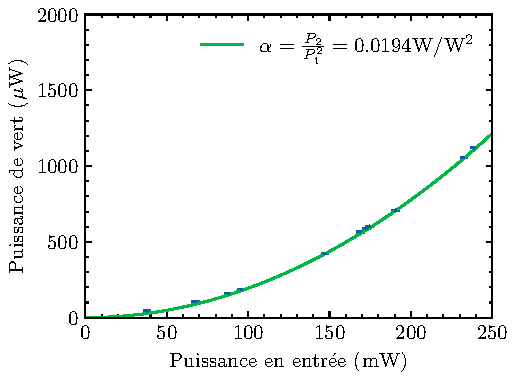
\includegraphics{../donnees/conversion basse puissance 82.5 C.pdf}
	\caption{Basse puissance}
	\label{fig:bp}
\end{figure}

\end{document}


